% The heading used to read "Grounding does not improve accuracy in the low-data regime
% either" -- an accuracy claim in one direction, which Sec. 5 and Table 2 decline to make,
% and which contradicted the caption below it once that caption was made to carry the
% no-claim rule. It names the sweep now, and the text carries the observation with its scope.
\subsection{The data-efficiency sweep, and what survives its confounds}
\label{sec:data-efficiency}
% Artifact: results/data_efficiency/summary.json via run_data_efficiency_summary.py
% over the Modal run (volume tgnn-e5, seed 42); ΔMAE = physics − DirectGNN.
% COMPRESSED 2026-08-20, from about 380 prose words to 190.  Nothing here is attributable -- the
% arms differ in capacity and in optimisation settings, the sweep is single-seed and non-monotone,
% and its endpoint does not reproduce the main comparison -- and the section said so at length.  A
% confound inventory longer than the result it disqualifies invites the question of why the result
% is in the submission at all.  What is kept is the observation that runs AGAINST this paper's own
% reading, and the reason nothing follows from it.  Table~\ref{tab:data-eff} and
% Fig.~\ref{fig:data-eff} are unchanged and carry the rest.
The strongest a-priori case for a physics prior is data scarcity: with few training molecules, an
inductive bias toward the correct factorisation should outperform a data-hungry black box. We test
it by subsampling the training set \emph{by solute} at fractions $0.05$--$1.0$ and training both
arms on the identical subsample (Table~\ref{tab:data-eff}, Fig.~\ref{fig:data-eff}, seed $42$). The
physics arm is worse at every fraction, and against the hypothesis the gap is \emph{smallest} at the
least data ($\Delta\mathrm{MAE}=+0.08$ at $5\%$) --- the one direction in this sweep that favours
the prior rather than this paper's reading of it.

Nothing in the sweep is attributable to the thermodynamic bottleneck, and no accuracy claim is made
from it. The two arms differ in capacity and in the per-arm optimisation settings of
\S\ref{sec:eval}, both are wider than the three-seed arms (hidden width $256$ and $128$ here, $64$
there), the sweep is single-seed with non-monotone physics-arm MAEs, and its endpoint does not
reproduce the main comparison: at fraction $1.0$ it gives $2.98$ against $1.97$ where the three-seed
runs of Table~\ref{tab:si-arms} give $1.7950$ against $1.7022$, a $\Delta\mathrm{MAE}$ an order of
magnitude apart ($+1.01$ here, $+0.09$ there). Both arms are worse than their three-seed
counterparts and the physics arm much the more so ($+1.18$ against $+0.27$ MAE), so the trend
measures how a light per-fraction budget interacts with training-set size at least as much as how a
physics prior does. The one inverting metric is top-1 solvent ranking ($0.42$ against $0.23$ at
$5\%$), which does not translate into lower error.

\begin{table}[t]
\centering
\caption[The data-efficiency sweep]{Data-efficiency sweep (train subsampled by solute, fixed scaffold test,
seed 42). $\Delta\mathrm{MAE}=\mathrm{MAE(physics)}-\mathrm{MAE(direct)}$.}
\label{tab:data-eff}
\resizebox{\columnwidth}{!}{%
\begin{tabular}{lrrrrr}
\toprule
train fraction & \multicolumn{2}{c}{MAE} & $\Delta\mathrm{MAE}$ & \multicolumn{2}{c}{$R^2$} \\
\cmidrule(lr){2-3}\cmidrule(lr){5-6}
(by solute) & physics & direct & (phys$-$dir) & physics & direct \\
\midrule
$0.05$ & $2.28$ & $2.20$ & $+0.08$ & $-0.09$ & $+0.07$ \\
$0.10$ & $2.44$ & $2.07$ & $+0.37$ & $-0.25$ & $+0.15$ \\
$0.25$ & $2.93$ & $1.81$ & $+1.12$ & $-0.75$ & $+0.38$ \\
$0.50$ & $3.12$ & $1.98$ & $+1.14$ & $-0.98$ & $+0.22$ \\
$1.00$ & $2.98$ & $1.97$ & $+1.01$ & $-0.79$ & $+0.22$ \\
\bottomrule
\end{tabular}}
\end{table}

\begin{figure}[t]
\centering
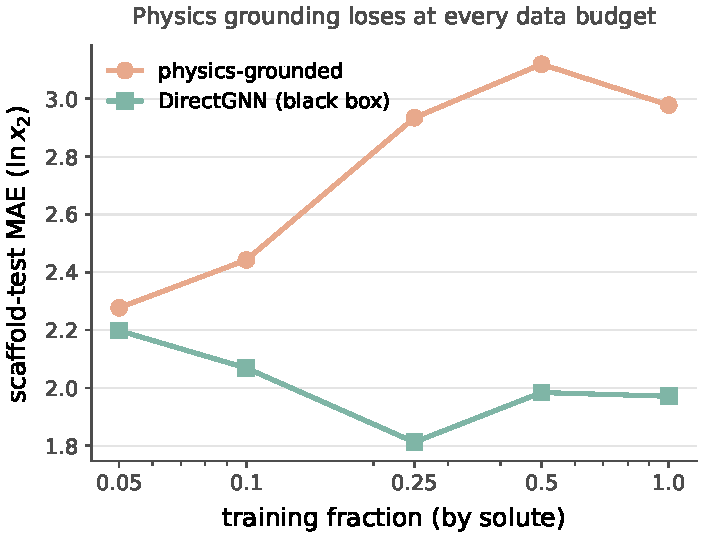
\includegraphics[width=\linewidth]{figs/fig_data_efficiency.pdf}
\caption[The data-efficiency curve]{Data-efficiency curve: scaffold-test MAE of the physics-grounded arm (salmon) and of
DirectGNN (teal) at five training-data fractions, one seed. The plotted values are the MAE columns
of Table~\ref{tab:data-eff}.}
\label{fig:data-eff}
\end{figure}
